\chapter{Alternative Methode}

Als alternative Methode zur Klassifizierung der 4 Klassen wird ebenfalls ein
neuronales Netz verwendet. Es erwies sich als äußerst schwierig, für diese
Problemstellung einen Lösungsansatz zu finden, der auf die Verwendung
neuronaler Netze verzichten kann. Wie zu Beginn dieser Arbeit bereits erwähnt,
gehört dieser Aufgabentyp zu den Aufgaben, die für Computer mit herkömmlichen
Methoden schwierig zu lösen sind.
Wie in Abschnitt~\ref{sec:netze} bereits beschrieben, eignen sich CNN am besten
zur Bilderkennung. Die Alternativmethode soll eine deutlich einfachere Lösung
darstellen, die einerseits zeigen soll, ob eine Lösung des Problems so möglich
ist und damit andererseits die \textit{performance} der Hauptarchitektur
relativieren. Daher verzichtet die Alternativmethode gänzlich auf CNN.
Außerdem wird der Datensatz so weit herunterskaliert, dass das Training auf
einem herkömmlichen PC in vertretbarer Rechenzeit durchgeführt werden kann.
%
\begin{figure}[h!]
  \subcaptionbox{Auf eine Größe von $50\text{px}\times100\text{px}$ skaliertes Beispielbild.}{\centering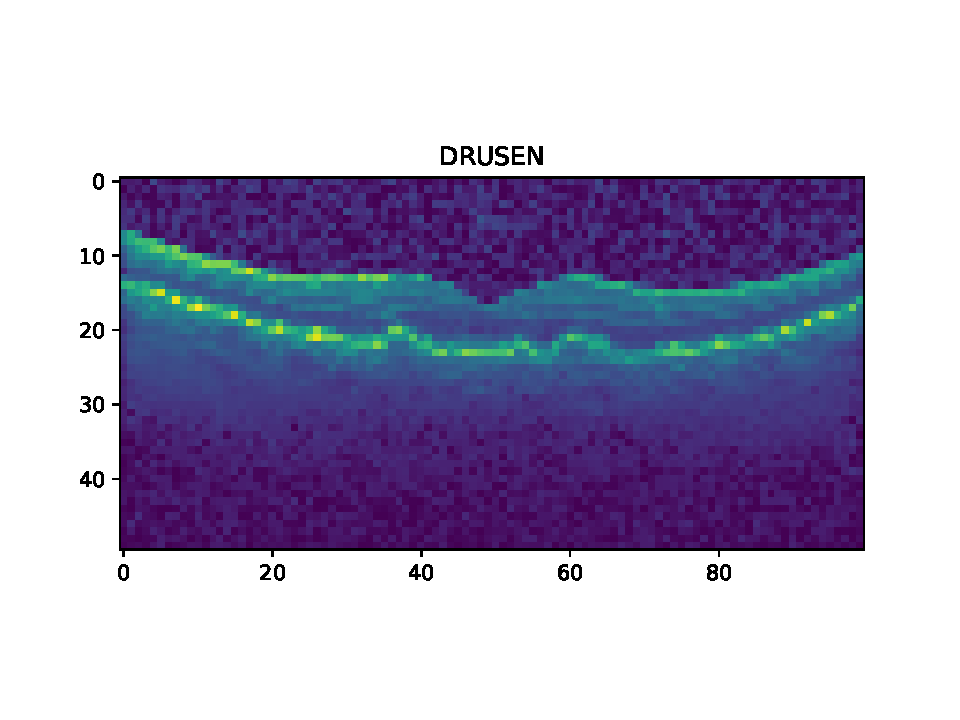
\includegraphics[width=0.5\linewidth]{Plots/image_0.pdf}}
  \hspace{5pt}
  \subcaptionbox{Die Verteilung der Mittelwerte aus dem \textit{Pooling} dieses Bildes.}{\centering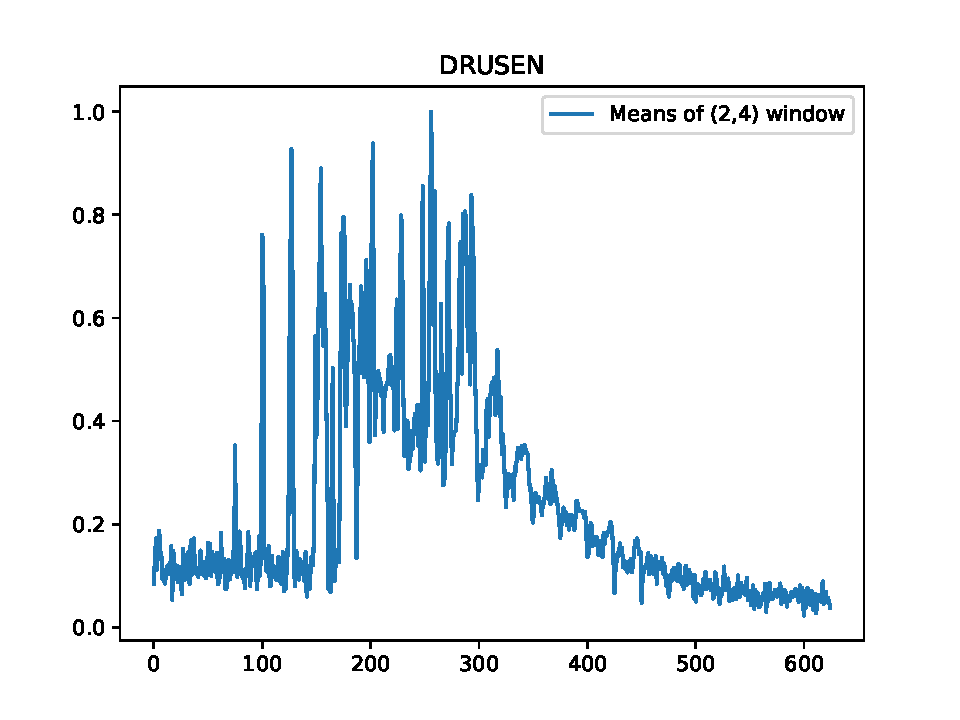
\includegraphics[width=0.5\linewidth]{Plots/distr.pdf}}
  \caption{Veranschaulichung der Datenskalierung für die Alternativmethode. Die Bilder werden zugeschnitten, skaliert und einem \textit{AveragePooling} unterzogen.}
  \label{fig:alter}
\end{figure}
%
Für diese Methode haben wir es uns zu Nutze gemacht, dass das Erkennen der
Krankheiten hauptsächlich im Bildmittelpunkt stattfindet. Die OCT Aufnahmen
sind verständlicherweise auf die Iris zentriert aufgenommen.
Daher wird das Bild zunächst zugeschnitten. Dazu werden die Pixelwerte auf eine
Achse projiziert, indem zeilenweise aufsummiert wird. In dieser Verteilung
lässt sich ein Maximum finden, welches als Mittelpunkt des Bildes dient.
Von diesem Mittelpunkt aus wird das Bild auf eine Größe von lediglich
$50\text{px}\times100\text{px}$ zugeschnitten. Dies reduziert die Dateigröße
und damit auch die Anzahl der \textit{input features} bereits etwa um einen
Faktor $30$.
Das so entstandene Bild wird schließlich einem \textit{Pooling} unterzogen.
Dazu wird in einem Fenster aus $2\times4$ Pixeln der Mittelwert berechnet und
dieser einzelne Wert gespeichert. Das Verfahren ist in
Abbildung~\ref{fig:alter} veranschaulicht. \\
Der so generierte Datensatz wird dann einem vollständig vernetzten Netz aus
Dichtelagen zum Training bereitgestellt. Die Architektur dieses Netzes ist in
XXX dargestellt.\\
Es handelt sich hierbei um ...\\
Die hierzu verwendete Architektur ist das Ergebnis einer intensiven
Optimierungsstudie. Durch die Skalierung des Datensatzes und die Verwendung
eines deutlich kleineren Netzes kann die Rechenzeit für das Training eines
Netzes stark reduziert werden. Dies ermöglicht auch eine intensive Suche nach
der besten Hyperparameterkonfiguration. Dazu wurden die Anzahl der Dichtelagen
in Kombination mit der Anzahl der Filter der einzelnen Dichtelagen, die
Aktivierungsfunktion in den Dichtelagen, sowie die Aktivierungsfunktion der
letzten Lage, sowie die Raten für die \textit{Dropout} Lagen variiert. So
konnten insgesamt mehr als $120$ Modellarchitekturen getestet werden. Die
Architektur mit der höchsten \textit{performance} ist oben beschrieben.
